% This file was created by matlab2tikz.
%
%The latest updates can be retrieved from
%  http://www.mathworks.com/matlabcentral/fileexchange/22022-matlab2tikz-matlab2tikz
%where you can also make suggestions and rate matlab2tikz.
%
\definecolor{mycolor1}{rgb}{0.00000,1.00000,1.00000}%
\definecolor{mycolor2}{rgb}{0.00000,0.44700,0.74100}%
\definecolor{mycolor3}{rgb}{0.85000,0.32500,0.09800}%
\definecolor{mycolor4}{rgb}{0.92900,0.69400,0.12500}%
\definecolor{mycolor5}{rgb}{0.49400,0.18400,0.55600}%
%
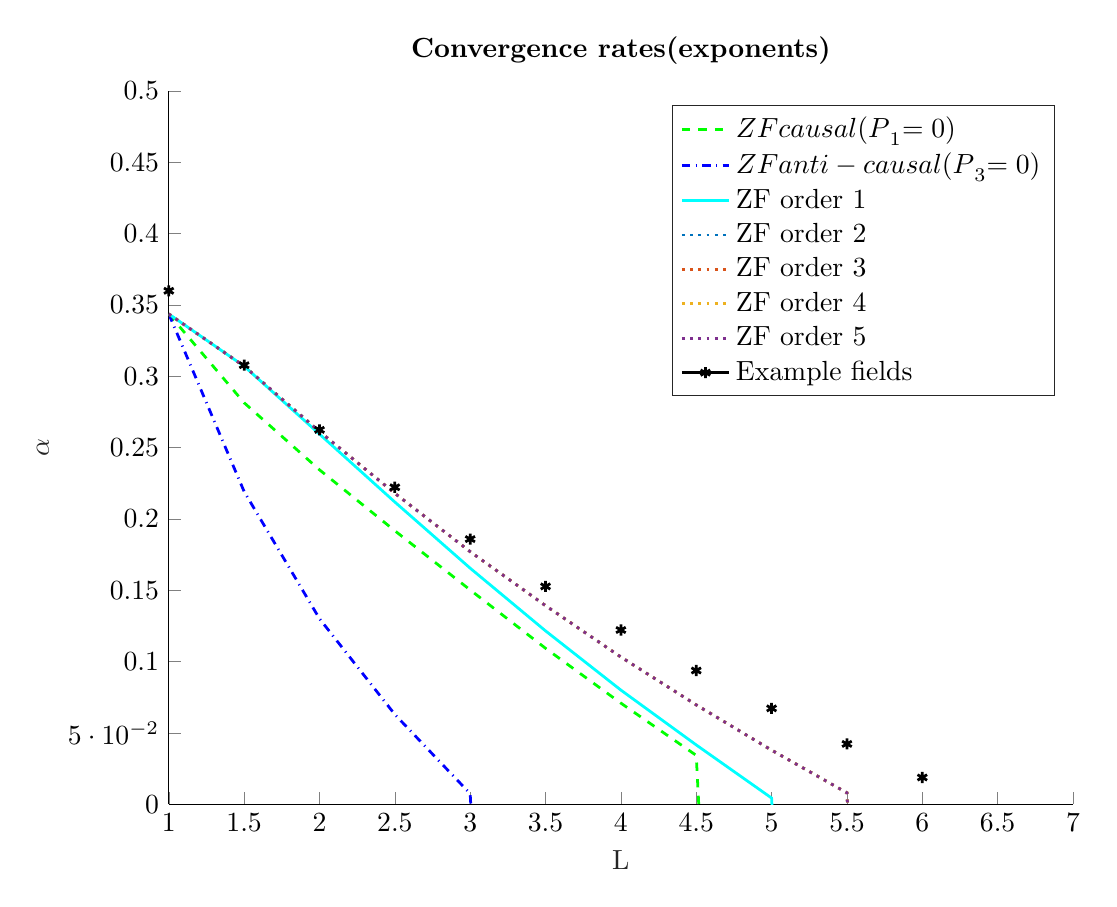
\begin{tikzpicture}

\begin{axis}[%
width=4.521in,
height=3.566in,
at={(0.758in,0.481in)},
scale only axis,
xmin=1,
xmax=7,
xlabel style={font=\color{white!15!black}},
xlabel={L},
ymin=0,
ymax=0.5,
ylabel style={font=\color{white!15!black}},
ylabel={$\alpha$},
axis background/.style={fill=white},
title style={font=\bfseries},
title={Convergence rates(exponents)},
axis x line*=bottom,
axis y line*=left,
legend style={legend cell align=left, align=left, draw=white!15!black}
]
\addplot [color=green, dashed, line width=1.0pt]
  table[row sep=crcr]{%
1	0.3436279296875\\
1.5	0.2813720703125\\
2	0.234375\\
2.5	0.191650390625\\
3	0.150146484375\\
3.5	0.1092529296875\\
4	0.07080078125\\
4.5	0.0341796875\\
5	-1\\
5.5	-1\\
6	-1\\
6.5	-1\\
7	-1\\
7.5	-1\\
8	-1\\
8.5	-1\\
9	-1\\
9.5	-1\\
10	-1\\
};
\addlegendentry{$\text{ZF causal (P}_\text{1}\text{=0)}$}

\addplot [color=blue, dashdotted, line width=1.0pt]
  table[row sep=crcr]{%
1	0.3436279296875\\
1.5	0.2191162109375\\
2	0.1300048828125\\
2.5	0.0628662109375\\
3	0.00732421875\\
3.5	-1\\
4	-1\\
4.5	-1\\
5	-1\\
5.5	-1\\
6	-1\\
6.5	-1\\
7	-1\\
7.5	-1\\
8	-1\\
8.5	-1\\
9	-1\\
9.5	-1\\
10	-1\\
};
\addlegendentry{$\text{ZF anti-causal (P}_\text{3}\text{=0)}$}

\addplot [color=mycolor1, line width=1.0pt]
  table[row sep=crcr]{%
1	0.3436279296875\\
1.5	0.3070068359375\\
2	0.2593994140625\\
2.5	0.2117919921875\\
3	0.1654052734375\\
3.5	0.1214599609375\\
4	0.0799560546875\\
4.5	0.04150390625\\
5	0.0042724609375\\
5.5	-1\\
6	-1\\
6.5	-1\\
7	-1\\
7.5	-1\\
8	-1\\
8.5	-1\\
9	-1\\
9.5	-1\\
10	-1\\
};
\addlegendentry{ZF order 1}

\addplot [color=mycolor2, dotted, line width=1.0pt]
  table[row sep=crcr]{%
1	0.3436279296875\\
1.5	0.3070068359375\\
2	0.26123046875\\
2.5	0.2178955078125\\
3	0.177001953125\\
3.5	0.13916015625\\
4	0.1031494140625\\
4.5	0.069580078125\\
5	0.037841796875\\
5.5	0.0079345703125\\
6	-1\\
6.5	-1\\
7	-1\\
7.5	-1\\
8	-1\\
8.5	-1\\
9	-1\\
9.5	-1\\
10	-1\\
};
\addlegendentry{ZF order 2}

\addplot [color=mycolor3, dotted, line width=1.0pt]
  table[row sep=crcr]{%
1	0.3436279296875\\
1.5	0.3070068359375\\
2	0.26123046875\\
2.5	0.2178955078125\\
3	0.177001953125\\
3.5	0.13916015625\\
4	0.1031494140625\\
4.5	0.069580078125\\
5	0.037841796875\\
5.5	0.0079345703125\\
6	-1\\
6.5	-1\\
7	-1\\
7.5	-1\\
8	-1\\
8.5	-1\\
9	-1\\
9.5	-1\\
10	-1\\
};
\addlegendentry{ZF order 3}

\addplot [color=mycolor4, dotted, line width=1.0pt]
  table[row sep=crcr]{%
1	0.3436279296875\\
1.5	0.3070068359375\\
2	0.26123046875\\
2.5	0.2178955078125\\
3	0.177001953125\\
3.5	0.13916015625\\
4	0.1031494140625\\
4.5	0.069580078125\\
5	0.037841796875\\
5.5	0.0079345703125\\
6	-1\\
6.5	-1\\
7	-1\\
7.5	-1\\
8	-1\\
8.5	-1\\
9	-1\\
9.5	-1\\
10	-1\\
};
\addlegendentry{ZF order 4}

\addplot [color=mycolor5, dotted, line width=1.0pt]
  table[row sep=crcr]{%
1	0.3436279296875\\
1.5	0.3070068359375\\
2	0.26123046875\\
2.5	0.2178955078125\\
3	0.177001953125\\
3.5	0.13916015625\\
4	0.1031494140625\\
4.5	0.069580078125\\
5	0.037841796875\\
5.5	0.0079345703125\\
6	-1\\
6.5	-1\\
7	-1\\
7.5	-1\\
8	-1\\
8.5	-1\\
9	-1\\
9.5	-1\\
10	-1\\
};
\addlegendentry{ZF order 5}

\addplot [color=black, line width=1.0pt, draw=none, mark=asterisk, mark options={solid, black}]
  table[row sep=crcr]{%
1	0.359877781991861\\
1.5	0.30771931207812\\
2	0.262397425883275\\
2.5	0.222141826976739\\
3	0.185818152359666\\
3.5	0.152649297281869\\
4	0.12207640065513\\
4.5	0.0936823881608809\\
5	0.0671467617957762\\
5.5	0.0422173233107017\\
6	0.0186916779750199\\
6.5	-0.00359531647237843\\
7	-0.0247803316318347\\
7.5	-0.0449778747672073\\
8	-0.0642849197875841\\
8.5	-0.0827843746763419\\
9	-0.100547722380696\\
9.5	-0.117637062795108\\
10	-0.13410671307487\\
};
\addlegendentry{Example fields}

\end{axis}
\end{tikzpicture}%